\item \textbf{{[}ALVL/9597/2018/P2/Q3{]} }
\begin{enumerate}
\item A binary tree is as follows: 
\begin{center}
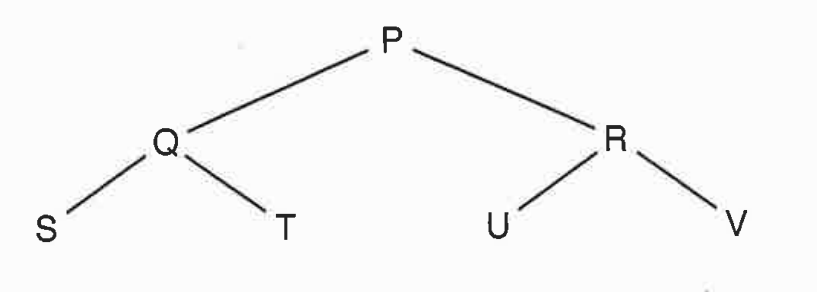
\includegraphics[width=0.5\paperwidth]{C:/Users/Admin/Desktop/Github/question_bank/LyX/static/img/9597-ALVL-2018-P2-Q3}
\par\end{center}
\begin{enumerate}
\item State the in-order sequence. \hfill{}{[}1{]}
\item State the pre-order sequence. \hfill{} {[}1{]}
\end{enumerate}
\item A 1D array, \texttt{Value}, stores a list of scores as follows:
\begin{center}
\begin{tabular}{|c|c|c|c|c|c|c|c|c|c|c|c|c|c|c|c|}
\hline 
Index & 0 & 1 & 2 & 3 & 4 & 5 & 6 & 7 & 8 & 9 & 10 & 11 & 12 & 13 & 14\tabularnewline
\hline 
Score & 2 & 6 & 15 & 23 & 36 & 48 & 50 & 58 & 64 & 69 & 74 & 79 & 86 & 92 & 99\tabularnewline
\hline 
\end{tabular}
\par\end{center}
\begin{enumerate}
\item Using a linear search, state how many comparisons will be required
to find the score of 64. \hfill{}{[}1{]}
\end{enumerate}
The following binary search algorithm could be used to search the
list of scores.

\noindent\begin{minipage}[t]{1\columnwidth}%
\texttt{01 Lower <- LowestIndex}

\texttt{02 Upper <- HighestIndex}

\texttt{03 REPEAT}

\texttt{04 \qquad{}Middle <- (Lower + Upper) DIV 2}

\texttt{05 \qquad{}IF SearchItem > Value{[}Middle{]}}

\texttt{O6 \qquad{}THEN}

\texttt{07 \qquad{}\qquad{}Lower <- Middle + l}

\texttt{08 \qquad{}ELSE}

\texttt{09 \qquad{}\qquad{}Upper <- Middle \textemdash{} l}

\texttt{10 \qquad{}ENDIF}

\texttt{11 UNTIL Value{[}Middle{]} = SearchItem OR Lower > Upper}

\texttt{12 OUTPUT \textquotedbl Score found at position\textquotedbl{}
Middle}%
\end{minipage}
\begin{enumerate}
\item[ii.] Score 80 is not in the list.

When searching for this score, state the values that will be examined.
\hfill{}{[}2{]}
\item[iii.] When searching for a score of 80, this algorithm outputs:

\texttt{Score found at position 12}

Describe how the algorithm gives this incorrect output. \hfill{}{[}2{]}
\item[iv.] Describe how the algorithm could be changed to give a suitable message
if the score is not in the list. \hfill{}{[}3{]}
\end{enumerate}
\end{enumerate}